\documentclass[border=4pt]{standalone}
\usepackage[T1]{fontenc}
\usepackage{helvet}\renewcommand{\familydefault}{\sfdefault}
\usepackage{tikz}
\usetikzlibrary{positioning,arrows.meta,fit,backgrounds,calc}
\definecolor{inC}{HTML}{2B6CB0}\definecolor{prC}{HTML}{3C8D5A}\definecolor{reC}{HTML}{7A4FB0}
\definecolor{evC}{HTML}{6B7280}\definecolor{ciC}{HTML}{C2571A}\definecolor{ouC}{HTML}{14181F}
\begin{document}
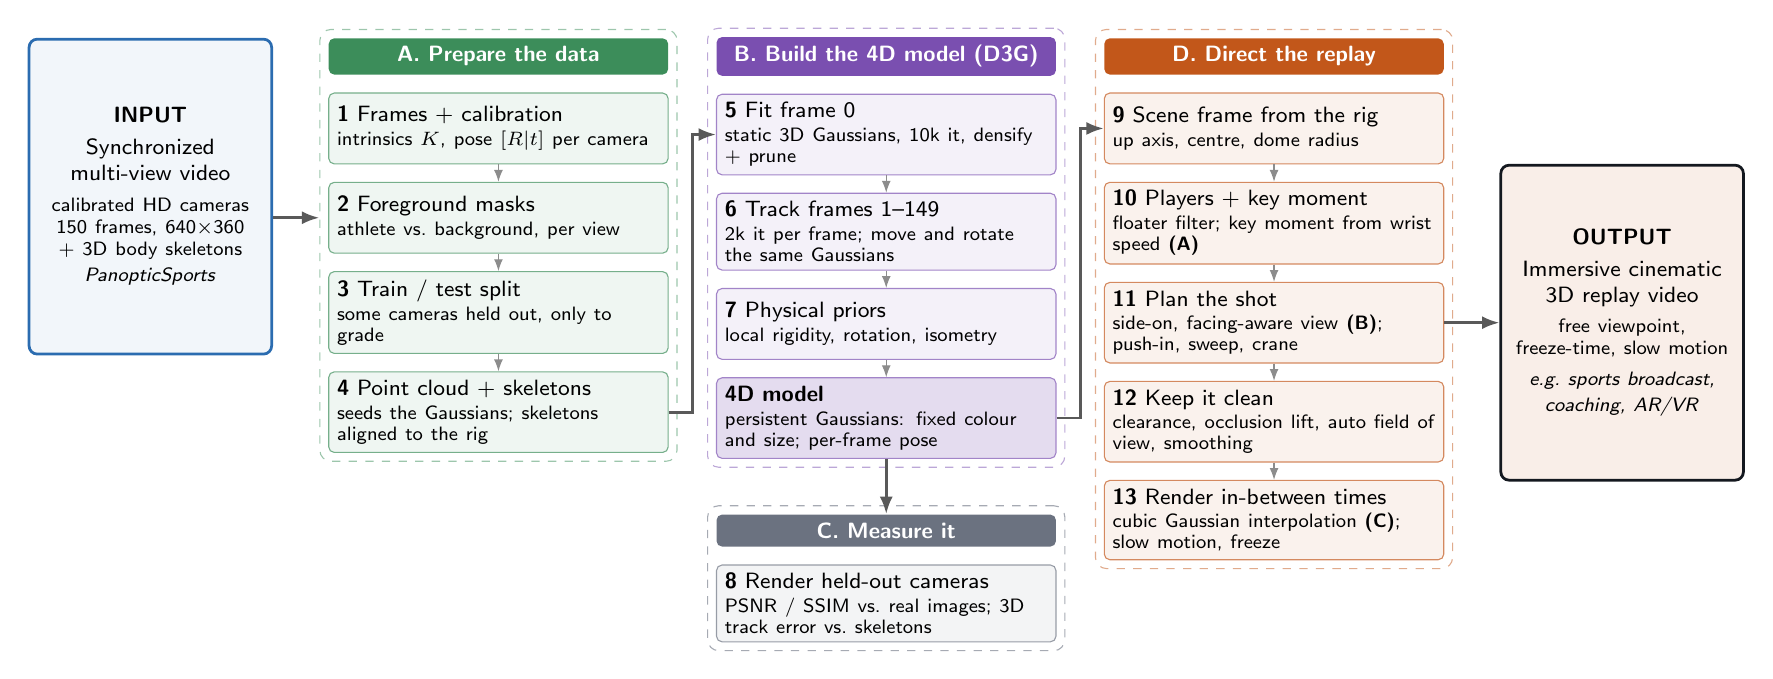
\begin{tikzpicture}[font=\footnotesize, node distance=2.2mm,
  st/.style={draw=#1!70, fill=#1!8, rounded corners=2pt, align=left, text width=41mm, inner sep=3pt, minimum height=9mm, execute at begin node={\hyphenpenalty=10000\exhyphenpenalty=10000\raggedright}},
  hd/.style={fill=#1, text=white, font=\footnotesize\bfseries, rounded corners=2pt, text width=41mm, align=center, inner sep=3pt},
  big/.style={draw=#1, line width=1pt, rounded corners=3pt, fill=#1!6, align=center, text width=28mm, inner sep=4pt},
  ar/.style={-{Latex[length=2.2mm]}, line width=1pt, draw=black!65}]
\node[big=inC, minimum height=40mm] (in) {\textbf{INPUT}\\[2pt]Synchronized\\multi-view video\\[3pt]\scriptsize calibrated HD cameras\\150 frames, 640$\times$360\\+ 3D body skeletons\\\textit{PanopticSports}};
\node[hd=prC, right=7mm of in.north east, anchor=north west] (ha) {A. Prepare the data};
\node[st=prC, below=of ha] (a1) {\textbf{1} Frames + calibration\par\vspace{1pt}{\scriptsize\linespread{0.95}\selectfont intrinsics $K$, pose $[R|t]$ per camera\par}};
\node[st=prC, below=of a1] (a2) {\textbf{2} Foreground masks\par\vspace{1pt}{\scriptsize\linespread{0.95}\selectfont athlete vs.\ background, per view\par}};
\node[st=prC, below=of a2] (a3) {\textbf{3} Train / test split\par\vspace{1pt}{\scriptsize\linespread{0.95}\selectfont some cameras held out, only to grade\par}};
\node[st=prC, below=of a3] (a4) {\textbf{4} Point cloud + skeletons\par\vspace{1pt}{\scriptsize\linespread{0.95}\selectfont seeds the Gaussians; skeletons aligned to the rig\par}};
\node[hd=reC, right=6mm of ha] (hb) {B. Build the 4D model (D3G)};
\node[st=reC, below=of hb] (b1) {\textbf{5} Fit frame 0\par\vspace{1pt}{\scriptsize\linespread{0.95}\selectfont static 3D Gaussians, 10k it, densify + prune\par}};
\node[st=reC, below=of b1] (b2) {\textbf{6} Track frames 1--149\par\vspace{1pt}{\scriptsize\linespread{0.95}\selectfont 2k it per frame; move and rotate the same Gaussians\par}};
\node[st=reC, below=of b2] (b3) {\textbf{7} Physical priors\par\vspace{1pt}{\scriptsize\linespread{0.95}\selectfont local rigidity, rotation, isometry\par}};
\node[st=reC, below=of b3, fill=reC!20] (b4) {\textbf{4D model}\par\vspace{1pt}{\scriptsize\linespread{0.95}\selectfont persistent Gaussians: fixed colour and size; per-frame pose\par}};
\node[hd=evC, below=7mm of b4] (hc) {C. Measure it};
\node[st=evC, below=of hc] (c1) {\textbf{8} Render held-out cameras\par\vspace{1pt}{\scriptsize\linespread{0.95}\selectfont PSNR / SSIM vs.\ real images; 3D track error vs.\ skeletons\par}};
\node[hd=ciC, right=6mm of hb] (hd) {D. Direct the replay};
\node[st=ciC, below=of hd] (d1) {\textbf{9} Scene frame from the rig\par\vspace{1pt}{\scriptsize\linespread{0.95}\selectfont up axis, centre, dome radius\par}};
\node[st=ciC, below=of d1] (d2) {\textbf{10} Players + key moment\par\vspace{1pt}{\scriptsize\linespread{0.95}\selectfont floater filter; key moment from wrist speed \textbf{(A)}\par}};
\node[st=ciC, below=of d2] (d3) {\textbf{11} Plan the shot\par\vspace{1pt}{\scriptsize\linespread{0.95}\selectfont side-on, facing-aware view \textbf{(B)}; push-in, sweep, crane\par}};
\node[st=ciC, below=of d3] (d4) {\textbf{12} Keep it clean\par\vspace{1pt}{\scriptsize\linespread{0.95}\selectfont clearance, occlusion lift, auto field of view, smoothing\par}};
\node[st=ciC, below=of d4] (d5) {\textbf{13} Render in-between times\par\vspace{1pt}{\scriptsize\linespread{0.95}\selectfont cubic Gaussian interpolation \textbf{(C)}; slow motion, freeze\par}};
\node[big=ouC, right=7mm of d3.east, anchor=west, minimum height=40mm, fill=ciC!10] (out) {\textbf{OUTPUT}\\[2pt]Immersive cinematic\\3D replay video\\[3pt]\scriptsize free viewpoint,\\freeze-time, slow motion\\[3pt]\textit{e.g.\ sports broadcast,}\\\textit{coaching, AR/VR}};
\begin{scope}[on background layer]
\node[draw=prC!50, dashed, rounded corners=4pt, fit=(ha)(a4), inner sep=3pt] (A) {};
\node[draw=reC!50, dashed, rounded corners=4pt, fit=(hb)(b4), inner sep=3pt] (B) {};
\node[draw=evC!60, dashed, rounded corners=4pt, fit=(hc)(c1), inner sep=3pt] (C) {};
\node[draw=ciC!50, dashed, rounded corners=4pt, fit=(hd)(d5), inner sep=3pt] (D) {};
\end{scope}
\draw[ar] (in.east |- a2.east) -- (a2.east -| A.west);
\draw[ar] (a4.east) -- ++(3mm,0) |- (b1.west);
\draw[ar] (b4.east) -- ++(3mm,0) |- (d1.west);
\draw[ar] (b4.south) -- (hc.north);
\draw[ar] (d3.east) -- (out.west);
\foreach \x/\y in {a1/a2,a2/a3,a3/a4,b1/b2,b2/b3,b3/b4,d1/d2,d2/d3,d3/d4,d4/d5} \draw[-{Latex[length=1.5mm]}, black!45] (\x.south) -- (\y.north);
\end{tikzpicture}
\end{document}
